% Drawing 144/09-3 -- folder 144, batch 09, archive page 165 (PDF page 166).
% Transcription: un cylindre ; au-dessous, un empilement de boîtes en perspective avec des axes $x$, $y$ ; à gauche, un cylindre sur lequel est collée une anse, avec une flèche de rotation et deux vecteurs $e_1$, $e_2$ ; plus bas, un parallélépipède hachuré avec les points $a_0, a_1, a_2, a_3$, $b_0, b_1, b_2, b_3$, $c_0, c_1, c_2, c_3$ ; à côté, $\sigma\varphi$ et $D_\sigma$ (un premier mot biffé).
% Kind: cylinder, stack of boxes, cylinder with a handle, hatched parallelepiped. Method 2 (schematic redraw from the facsimile). Status: partial.
% Notes: Most of the page; each of the four figures re-read on its own tight crop. Top right: the horizontal cylinder, its two end ellipses (the right one doubled, the inner trace in pencil) joined by the top and bottom lines. Under it, the stack of boxes in perspective: corners placed once and the edges drawn between them as he draws them, the top box (front face and the strokes behind it), the middle and the lower box with its thick front edge between two dots and thick left edge, the diagonal strokes of the middle box in pencil, the long x line from the dot to the right, the y stroke at the left, axes labelled y and x. Left: the cylinder with the handle glued on: the cylinder (left end ellipse, its rim, the long lines, the right end), the two arcs of the handle with their arrowheads, the rotation arrow above, the small loop on the cylinder, the vectors e_1, e_2 from their common point. Below: the parallelepiped with its corners a_0..a_3, b_0..b_3, c_0..c_3 placed once (dots where he inks them), thick edges as on the page with their arrowheads, the thin edges and the face a_3, a_2, a_1, a_0, and the left face hatched; beside it sigma phi and D_sigma. Labels \small. Strike-outs not drawn: the struck word before D_sigma. Still differs from the facsimile: the edges of the stack of boxes are a reading of an overinked sketch (several strokes there are doubled and some faint ones are left out); the hatching of the parallelepiped is drawn as a pattern on its left face, while on the page it is a tangle of strokes over the left part; the arcs of the handle are approximate. The formulas on the page are text. Redrawn 2026-11-09 (issue 128): to check again.
% Coordinates: 1 unit = 1 mm = 1/100 of the crop width (bbox in page fractions: [0.08, 0.08, 0.72, 0.68]).
% Redrawn by Claude (claude-opus-5-5), issue #73, 2026-11-09; not checked by a human; not compiled (no TeX in the session).
% Rights: reproduces part of the work -- behind RENDER_TRANSCRIPTS, never published by itself.
\documentclass[tikz,border=3pt]{standalone}
\usepackage{amsmath,amssymb}
\usetikzlibrary{patterns,arrows.meta}
\tikzset{pencil/.style={black!45}, struck/.style={black!35}, mark/.style={circle,draw,inner sep=1.3pt}, pt/.style={circle,fill,inner sep=0.9pt}, opt/.style={circle,draw,fill=white,inner sep=1.1pt}}
\begin{document}
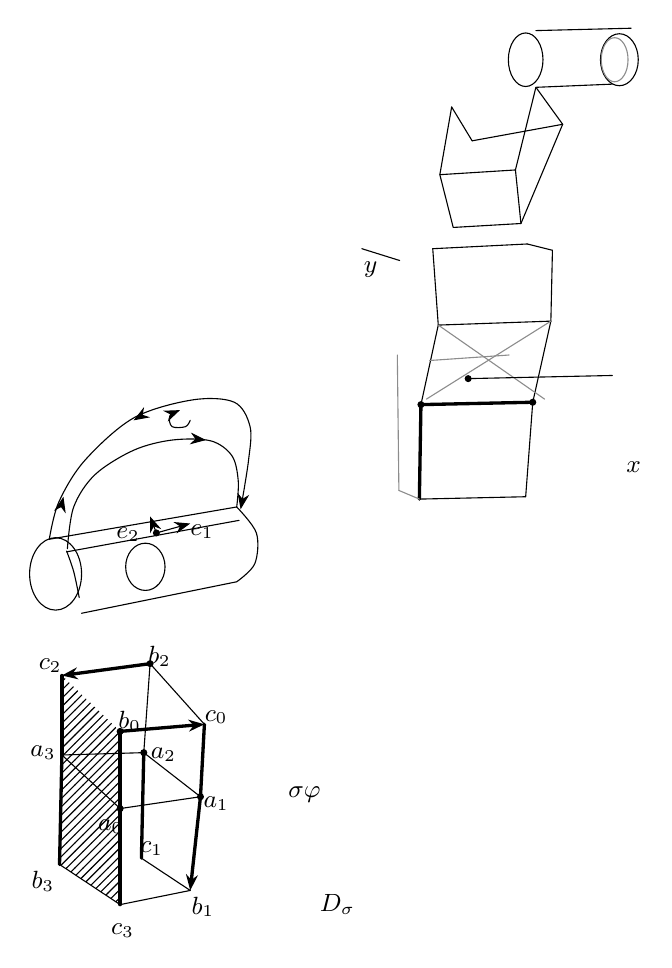
\begin{tikzpicture}[x=1mm,y=1mm,line cap=round,line join=round,font=\scriptsize]
\draw (80.2,-13.6) ellipse[x radius=2.2, y radius=3.4];
\draw (92.1,-13.6) ellipse[x radius=2.4, y radius=3.3];
\draw[pencil] (91.5,-13.6) ellipse[x radius=1.7, y radius=2.8];
\draw (81.5,-9.9) -- (93.6,-9.6);
\draw (81.6,-17.1) -- (91.2,-16.7);
\draw (69.3,-28.2) -- (78.9,-27.6) -- (79.6,-34.4) -- (71,-34.9) -- cycle;
\draw (69.3,-28.2) -- (70.8,-19.6);
\draw (70.8,-19.6) -- (73.4,-23.9);
\draw (73.4,-23.9) -- (84.9,-21.8);
\draw (81.5,-17.1) -- (84.9,-21.8);
\draw (84.9,-21.8) -- (79.6,-34.4);
\draw (81.5,-17.1) -- (78.9,-27.6);
\draw (68.4,-37.6) -- (80.4,-37);
\draw (80.4,-37) -- (83.6,-37.8);
\draw (68.4,-37.6) -- (69.1,-47.3);
\draw (83.6,-37.8) -- (83.4,-46.8);
\draw (69.1,-47.3) -- (83.4,-46.8);
\draw (69.1,-47.3) -- (66.9,-57.4);
\draw (83.4,-46.8) -- (81.1,-57.1);
\draw (66.7,-69.4) -- (80.2,-69.1);
\draw (80.2,-69.1) -- (81.1,-57.1);
\draw[very thick] (66.9,-57.4) -- (81.1,-57.1);
\draw[very thick] (66.9,-57.4) -- (66.7,-69.4);
\node[pt] at (66.9,-57.4) {};
\node[pt] at (81.1,-57.1) {};
\draw[pencil] (68,-51.8) -- (78.1,-51.1);
\draw[pencil] (63.9,-51.1) -- (64.1,-68.3);
\draw[pencil] (64.1,-68.3) -- (66.7,-69.4);
\draw[pencil] (69.1,-47.3) -- (82.6,-56.7);
\draw[pencil] (83.4,-46.8) -- (67.6,-56.7);
\draw (72.9,-54.1) -- (91.2,-53.7);
\node[pt] at (72.9,-54.1) {};
\draw (59.4,-37.6) -- (64.2,-39.1);
\node[inner sep=1pt] at (60.5,-40.2) {\small $y$};
\node[inner sep=1pt] at (93.9,-65.3) {\small $x$};
\draw (20.5,-78.9) ellipse[x radius=3.3, y radius=4.6];
\draw plot[smooth, tension=0.55] coordinates {(21.9,-76) (22.8,-78.6) (23.5,-81.9)};
\draw (19.7,-74.5) -- (43.5,-70.4);
\draw (21.9,-76.1) -- (43.8,-72.1);
\draw (23.8,-83.9) -- (43.5,-79.9);
\draw plot[smooth, tension=0.55] coordinates {(43.5,-70.4) (46,-73.7) (45.8,-77.6) (43.5,-79.9)};
\draw[-{Stealth[length=2mm]}] plot[smooth, tension=0.55] coordinates {(19.7,-74.5) (20.9,-69.8) (24.2,-64.5) (30.4,-59.1) (37.9,-56.8) (43.2,-57.1) (45.2,-60.2) (45,-64.5) (44,-70.7)};
\draw plot[smooth, tension=0.55] coordinates {(22,-75.7) (22.8,-70.4) (25.5,-66.3) (30.4,-63.2) (35.3,-61.9) (40.2,-62) (42.9,-63.9) (43.7,-67.1) (43.5,-70.4)};
\draw[-{Stealth[length=2mm]}] (30.9,-59.1) -- (30.4,-59.4);
\draw[-{Stealth[length=2mm]}] (38.6,-61.8) -- (39.6,-61.9);
\draw[-{Stealth[length=2mm]}] (21.2,-70.4) -- (21.5,-69.1);
\draw[{Stealth[length=2mm]}-] plot[smooth, tension=0.55] coordinates {(36.3,-58.1) (35,-58.9) (35.3,-60.2) (37,-60.2) (37.6,-59.4)};
\draw (31.9,-78) ellipse[x radius=2.5, y radius=3];
\draw[-{Stealth[length=2mm]}] (33.3,-73.7) -- (37.6,-72.5);
\draw[-{Stealth[length=2mm]}] (33.3,-73.7) -- (32.5,-71.6);
\node[pt] at (33.3,-73.7) {};
\node[inner sep=1pt] at (39.1,-73.5) {\small $e_1$};
\node[inner sep=1pt] at (29.7,-73.9) {\small $e_2$};
\draw[-{Stealth[length=2mm]},very thick] (32.5,-90.3) -- (21.3,-91.8);
\draw[-{Stealth[length=2mm]},very thick] (28.7,-98.9) -- (39.4,-98);
\draw[very thick] (21.3,-91.8) -- (21.3,-101.9);
\draw[very thick] (21.3,-101.9) -- (21,-115.8);
\draw[very thick] (39.4,-98) -- (38.9,-107.2);
\draw[very thick] (28.7,-98.9) -- (28.7,-108.7);
\draw[very thick] (28.7,-108.7) -- (28.7,-120.9);
\draw[very thick] (31.7,-101.6) -- (31.4,-115);
\draw[-{Stealth[length=2mm]},very thick] (38.9,-107.2) -- (37.6,-119.1);
\draw (32.5,-90.3) -- (31.7,-101.6);
\draw (21,-115.8) -- (28.7,-120.9);
\draw (28.7,-120.9) -- (37.6,-119.1);
\draw (31.4,-115) -- (37.6,-119.1);
\draw (21.3,-101.9) -- (31.7,-101.6);
\draw (31.7,-101.6) -- (38.9,-107.2);
\draw (21.3,-101.9) -- (28.7,-108.7);
\draw (28.7,-108.7) -- (38.9,-107.2);
\draw (32.5,-90.3) -- (39.4,-98);
\fill[pattern=north east lines] (21.3,-91.8) -- (28.7,-98.9) -- (28.7,-120.9) -- (21,-115.8) -- cycle;
\node[pt] at (32.5,-90.3) {};
\node[pt] at (28.7,-98.9) {};
\node[pt] at (31.7,-101.6) {};
\node[pt] at (28.7,-108.7) {};
\node[pt] at (38.9,-107.2) {};
\node[inner sep=1pt] at (19.8,-90.6) {\small $c_2$};
\node[inner sep=1pt] at (33.7,-89.4) {\small $b_2$};
\node[inner sep=1pt] at (29.9,-97.6) {\small $b_0$};
\node[inner sep=1pt] at (40.9,-97.1) {\small $c_0$};
\node[inner sep=1pt] at (18.9,-101.6) {\small $a_3$};
\node[inner sep=1pt] at (34.2,-101.9) {\small $a_2$};
\node[inner sep=1pt] at (27.5,-111) {\small $a_0$};
\node[inner sep=1pt] at (40.9,-108.1) {\small $a_1$};
\node[inner sep=1pt] at (32.7,-113.8) {\small $c_1$};
\node[inner sep=1pt] at (18.9,-117.9) {\small $b_3$};
\node[inner sep=1pt] at (39.2,-121.2) {\small $b_1$};
\node[inner sep=1pt] at (29,-124.2) {\small $c_3$};
\node[inner sep=1pt] at (52.1,-106.9) {\small $\sigma\varphi$};
\node[inner sep=1pt] at (56.3,-120.9) {\small $D_\sigma$};
\end{tikzpicture}
\end{document}
